\documentclass[a4paper]{network-pa}

\usepackage{graphicx}
\usepackage{mathtools}
\usepackage{tabularx}
\usepackage{color}
\usepackage{algc}
\usepackage{array}
\usepackage{float}
\renewcommand{\labelenumi}{\arabic{enumi}. }
%\usepackage[table,xcdraw]{xcolor}
\usepackage[utf8]{inputenc}
\usepackage[table]{xcolor}
\usepackage{tablefootnote}
 
\definecolor{codegray}{gray}{0.9}
\newcommand{\code}[1]{\lr{\colorbox{codegray}{\texttt{#1}}}}
\newcommand{\notice}{
\emph{
نکته:
}}
\newfontfamily{\adaadNiloo}[Script=Parsi,Language=Parsi]{XB Niloofar}

\hypersetup{
	pdfsubject = {Operating Systems (CE 40-424) Homework},
	pdftitle = {Personal Assignment 0 (A0)}
}

\usepackage{xepersian}
\settextfont{XB Niloofar}

\graphicspath{{Pics/}}

\newfontfamily{\adaadNiloo}[Script=Parsi,Language=Parsi]{XB Niloofar}
\adaadNiloo

\title{
تمرین صفرم
}

\author{
محمدحامد فتحی
}

\thanksta{
با سپاس از 
}

\date{
پاییز ۱۳۹۶
}

\begin{document}	
\maketitle\thispagestyle{fancy}
\textbf{ {\Large اهداف تمرین}}
\RTL{
\begin{itemize}
\item
راه اندازی پیش نیازهای انجام تمارین
\item
آشنایی با چند ابزار مفید برای تولید و رفع باگ کد
\item
آشنایی با نحوه ارسال تمارین
\end{itemize}
}

\section{مقدمه}
این تمرین شامل سه بخش اصلی میشود که عبارتند از: نصب پیشنیازهای انجام تمارین، آشنایی با چند ابزار مفید و چند تمرین ابتدایی و ساده.
\newpage
\section
{
\textbf{ {\Large 
بخش اول: راه اندازی مقدمات
}}}

\subsection{Github}
تمامی تمارین فردی و گروهی شما از طریق سامانه Github دریافت می گردد. بنابراین شما به یک حساب کاربری در Github نیازمندید.
تیم دستیاران تمرین برای تمامی تمارین مخازن خصوصی می سازند و در اختیارتان فرار می دهند.

\subsection{Vagrant}
تیم دستیاران تمرین تصویری
\LTRfootnote{image}
از ماشین مجازی لازم جهت تست و اجرای تمامی کدها فراهم کرده است. Vagrant ابزاری جهت مدیریت ماشینهای مجازی است. شما میتوانید 
از Vagrant  برای دانلود و اجرای تصویر داده شده استفاده کنید.

\notice{
اگر تمایلی به استفاده از Vagrant نداشتید میتوانید از لینک زیر برروی Github ماشین مجازی را دریافت کرده و با نرم افزار مورد نظر خود اجرا کنید.
}

\notice{
اگر از ویندوز استفاده می کنید، میتوانید از این گامها عبور کنید. در ادامه در خصوص راه اندازی برروی ویندوز توضیحاتی بیان خواهد گردید.
}

\begin{itemize}
\item
راه اندازی Vagrant نیازمند نصب و راه ندازی VirtualBox است. بنابراین شما نیاز دارید که مناسب ترین ورژن آنرا از اینجا دانلود و نصب کنید.
در کلاس درس بیشتر در مورد ماشینهای مجازی توضیح داده خواهد شد، اما فعلا میتوانید تصور کنید که منظور از یک ماشین مجازی، نسخه نرم افزاری یک سخت افزار واقعی است.
\item
نسخه مناسب Vagrant را از اینجا نصب کنید. 
\item
دستورهای زیر را در ترمینال تایپ کنید.
\begin{flushleft}
\code{mkdir cs162-vm}
\code{cd cs162-vm}
\code{vagrant init cs162/spring2017}
\code{vagrant up}
\code{vagrant ssh}
\end{flushleft}
توجه کنید که دستور up به اتصال اینترنت نیازمند است.
\item
می بایست تمامی دستورهای Vagrant را از دایرکتوری cs162-vm اجرا کنید و مواظب باشید که این دایرکتوری را پاک نکنید.
\item
به منظور متوقف کردن ماشین مجازی میتوانید از دستور \begin{flushleft}
\code{vagrant halt}
\end{flushleft} استفاده کنید.
\end{itemize}

\subsubsection{
\lr{Windows}:
}
از آنجایی که سیستم عامل ویندوز از ssh پشتیبانی نمیکند، دانبود و نصب Cygwin میتواند گزینه مناسبی باشد. شما میتوانید از اینجا راهنمای نصب تنظیمات Vagrant در ویندوز به کمک Cygwin را مشاهده نمایید.

\subsubsection{
\lr{Troubleshooting Vagrant}:
}
اگر دستور \begin{flushleft}
\code{vagrant up}
\end{flushleft} با مشکل مواجه شد، تلاش کنید تا با اجرای دستور \begin{flushleft}
\code{vagrant provision}
\end{flushleft} مشکل را برطرف نمایید.
اگر کماکان مشکل برطرف نشد، برای تلاش آخر میتوانید به کمک دستور \begin{flushleft}
\code{vagrant destroy}
\end{flushleft} ماشین مجازی خود را از کار بیندازید و مجددا تلاش کنید تا دستور \begin{flushleft}
\code{vagrant up}
\end{flushleft} اجرا شود.

\subsubsection{
\lr{Git Name و Email}:
}
دستورهای زیر را اجرا کنید تا تنظیماتی که برای کامیت هایتان استفاده میکنید برقرار گردد.

\begin{flushleft}
\code{git config --global user.name "Your Name"}
\code{git config --global user.email "Your Email"}
\end{flushleft}

\subsubsection{
\lr{ssh-key}:
}
در این مرحله نیاز دارید که کلیدهای ssh خود را به منظور شناسایی Github از درون ماشین مجازیتان مظابق زیر تنظیم کنید.

\begin{flushleft}
\code{ssh-keygen -N "" -f ~/.ssh/id_rsa}
\code{cat ~/.ssh/id_rsa.pub}
\end{flushleft}

دستور اول یک جفت کلید ssh برایتان تولید میکند. دستور دوم کلید عمومیتان را در صفحه نمایش نشان میدهد. شما میبایست به Github ورود کرده و سپس از این قسمت کلید عمومیتان را به حساب خود بفزایید. کلید شما باید با عبارت “ssh-rsa” شروع شده و با “vagrant@development” پایان یافته باشد.

\subsubsection{
\lr{مخازن}:
}
شما به دومخزن خصوصی در این درس دسترسی دارید. به عبارت دیگر به یک مخزن برای تمرینهای فردی و به یک مخزن برای تمرینهای گروهی دسترسی دارید.
ساختار کدهای تمارین فردی را از اینجا و تمارین گروهی را از اینجا میتوانید مشاهده کنید. این دو مخزن در حال حاضر در آدرس ~/code/personal و ~/code/group از ماشین مجازیتان قرار دارند.
میتوانید از قابلیت “Remotes” در گیت بهره ببیرد تا ساختار کدها را در صورت تغییر یا بروزرسانی آنها از مخازن ما دریافت کنید. همچنین به کمک push کدهای خود را به مخازن نظیرشان ارسال کنید. درواقع قابلیت “Remotes” به شما این امکان را میدهد که مخازن Github را به مخازن محلی خود متصل کنید. درحال حاضر یک remote به نام “staff” قرار داده شده است که به مخازن ما در Github اشاره می کند.
به منظور افزودن یک remote جدید به ماشین مجازیتان، پیشنهاد می شود گامهای زیر را طی کنید:

\begin{itemize}
\item
در ابتدا به مخزن مربوط به تمارین فردی بروید:\begin{flushleft}
\code{cd ~/code/personal}
\end{flushleft}
\item
سپس مخزن تمارین فردیتان در Github را مشاهده کنید و آدرس SSH clone را بیابید. اگر آدرس فرمتی مشابه “git@github.com:Berkeley-CS162/...” داشت به سراغ گام بعد بروید.
\item
به کمک دستور \begin{flushleft}
\code{git remote add personal YOUR_GITHUB_CLONE_URL}
\end{flushleft} remote را اضافه کنید.
میتوانید اطلاعات آن را از طریق دستورهای زیر مشاهده کنید:
\begin{flushleft}
\code{git remote -v}
\code{git remote show personal}
\end{flushleft}
\item
ساختار را pull کرده ، یک کامیت تستی ساخته و آنرا push کنید
\begin{flushleft}
\code{git pull staff master}
\code{touch test_file}
\code{git add test_file}
\code{git commit -m "Added a test file."}
\code{git push personal master}
\end{flushleft}
\end{itemize}

\subsection{ویرایش کد در ماشین مجازی}
ماشین مجازی برای آنکه بتوانید پوشه home از vagrant فایلهایتان را ویریایش کنید، از سرور SMB استفاده میکند. به کمک این سرور میتوانید از هر ویرایشگر متنی که بر روی سیستم خود دارید استفاده کنید تا کدها را ویرایش کرده و دستورهای git را از درون ماشین مجازی خود اجرا کنید.
این روش پیشنهادی برای کار برروی کدها در این درس است، اما شما آزادید که از هر روشی که به نظرتان مناسب تر است استفاده کنید.

\subsubsection{
\lr{Windows}:
}
\begin{itemize}
\item
file browser را باز کرده و دکمه Ctrl L را فشار دهید تا برروی location bar focus کنید.
\item
عبارت “\\192.168.162.162\vagrant” را تایپ کرده و دکمه Enter را فشار دهید.
\item
نام کاربری و رمز عبور هر دو برابر است با: vagrant
\end{itemize}
\subsubsection{
\lr{Mac OS X}:
}
\begin{itemize}
\item
Finder را باز کنید.
\item
قسمت “Go → Connect to Server...” را انتخاب کنید.
\item
آدرس سرور برابر است با: “smb://192.168.162.162/vagrant”.
\item
نام کاربری و رمز عبور هر دو برابر است با: vagrant
\end{itemize}
\subsubsection{
\lr{Linux}:
}
از هر SMB client میتوانید استفاده کنید تا به “192.168.162.162/vagrant” متصل شوید.
نام کاربری و رمز عبور برابر است با: vagrant

\subsection{پوشه های اشتراکی}
پرونده /vagrant در ماشین مجازیتان به پوشه خانه\LTRfootnote{image} سیستم اصلیتان متصل شده است. اگر نیاز داشتید میتوانید از این اتصال استفاده کنید، اگرچه متود SMB که در قسمت قبل گفته شد پیشنهاد می گردد.
\newpage
\section
{
\textbf{ {\Large 
بخش دوم: چند ابزار مفید
}}}
در اسن بخش با چند ابزار مفید آشنا می شوید که معمولا در جعبه ابزار هر سامانه حمله کننده ای معمولا یافت می شود. از میان این ابزار یادگیری git و make الزامی هستند، زیرا بدون کسب دانش کافی از این ابزار قادر نخواهید بود کد خود را کامپایل نموده و سپس ارسال کنید. سایر ابزار یا در جهت رفع باگ به کار میروند یا در جهت چندوظیفگی\LTRfootnote{multitasking} با کارای بیشتر مورد استفاده قرار می گیرند.
\notice{
تمامی این ابزارها بر روی ماشین مجازی نصب گردیده اند.
}

\subsection{Git}
یک برنامه version control است که به کمک آن میتوانید روند کدها را دنبال کنید. GitHub یکی از سامانه های تحت وب است که امکان hosting کدهای شما را برایتان فراهم می کند. درواقع این سامانه فضای تعاملی و اشتراک گذاری کدها را فراهم ساخته است.
اگر چه تا این مرحله شما تنظیمات مقدماتی را انجام داده اید، اما تسلط شما به قابلیتهای git میتواند در طول این درس به کمک شما بیاید، خصوصا هنگامی که با هم گروهی هایتان تمرین را انجام می دهید.
اگر مایلید که سطح دانش خودتان را نسبت به گیت افزایش دهید میتوانید اینجا را مشاهده کنید.

\subsection{make}
make ابزاری است که به صورت خودکار برنامه های اجرایی و کتابخانه ها را از کد منبع تولید می کند و این کار را به کمک خواندن فایل Makefile انجام می دهد. Makefile تعیین می کند که چگونه به برنامه هدف دسترسی پیدا کند. به این صورت که لیست تمامی وابستگی ها\LTRfootnote{dependency} را در آن قرار می هدید و make با پیمیایش آنها برنامه اجرایی شما را تولید می کند.
متاسفانه make syntax بسیار بدی دارد که اگر به صورت درست از آنها استفاده نکنید برای فهم آنها دچار مشکل خواهید شد.
بنابراین توصیه می شود از اینجا آموزش لازم را فرا بگیرید.
فعلا ما از ساده ترین فرم make که نیازی به Makefile ندارد استفاده می کنیم. بنابراین با اجرای دستور زیر میتوانید به راحتی کامپایل کرده به wc.c متصل شوید.\begin{flushleft}
\code{make wc}
\end{flushleft}
این دستور یک فایل اجرایی ایجاد کرد که شما میتوانید اجرایش کنید. حال دستور زیر را اجرا کنید:
\begin{flushleft}
\code{./wc wc.c}
\end{flushleft}
تفاوت دستور بالا با دستوری که در ادامه می آید چیست؟ (راهنمایی: ابتدا دستور “which wc” را اجرا کنید.)
\begin{flushleft}
\code{wc wc.c}
\end{flushleft}

تمرین اول شما این خواهد بود که wc.c را به گونه ای تغییر دهید که تعداد کلمات را با توجه به ویژگیهای “man wc” پیاده سازی کند و در آن تنها نیاز دارید که از یک فایل ورودی پشتیبانی کنید(یا STDIN اگر هیچ ویژگی تعیین نشده بود).
توجه کنید که wc در OS X کاملا متفاوت از Ubuntu عمل می کند، بنابراین انتظار می رود که رفتار آن را در Ubuntu دنبال کنید.

\subsection{gdb}
دیباگ کردن برنامه های با زبان C بسیار سخت است اما خوشبختانه gdb امکان دیباگ کردن آسان را فراهم نموده است. اگر شما برنامه هایتان را با پرچم\LTRfootnote{flag} خاص -g کامپایل کنید و برنامه را داخل gdb اجرا کنید علاوه بر stack trace میتوانید متغیرها را inspect کنید، غییر دهید، کد را متوقف کنید و ... .
gdb ساده امکانات کمی دارد، به همین دلیل cgdb روی ماشین مجازی برایتان نصب شده است که یک سری قابلیتها از قبیل syntax highlighting را داراست. در cgdb میتوانید با استفاده از i و ESC بین پنجره\LTRfootnote{pane} های بالایی و پایینی switch کنید.
همچنین gdb میتواند پردازه های جدید را شروع کند و به پردازه های درحال اجرا ملحق کند.
برای یادگیری gdb پیشنهاد می کنیم اینجا را مشاهده کنید. البته مستند اصلی gdb نیز علی رغم طولانی بدن مفید است.
برای یادگیری بیشتر تلاش کنید با wcتان کار کنید. با پرچم\LTRfootnote{flag} -g برنامه تان را کامپایل کنید. برنامه را از طریق gdb شروع کنید کنید و یک نقطه وقفه\LTRfootnote{break point} بر سر main بگذارید. سپس برنامه را تا آنجا اجرا کنید و دستورهای مختلف را تمرین کنید. بفهمید که چگونه آرگومان های خط فرمان را میتوان pass داد. متغیرهای محلی اضافه کنید و مقادیر\LTRfootnote{value} نظیرشان را پیدا کنید. step ، next و break را فرابگیرید.

\subsection{tmux}
یک multiplexer مربوط به terminal است که چندین tab مربوط به terminalرا شبیه سازی می کند اما آنها را در یک session از terminal نمایش می دهد. البته این چند tab را هنگام ssh به ماشین مجازی حفظ می کند.
شما میتوانید یک session جدید را با دستور \begin{flushleft}
\code{tmux new -s <session_name>}
\end{flushleft} ایجاد کنید. سپس میتوانید با فشار دادن \begin{flushleft}
\code{ctrl-b + c}
\end{flushleft} یک پنجره\LTRfootnote{window} جدید ایجاد کنید و با فشار دادن \begin{flushleft}
\code{ctrl-b + n}
\end{flushleft} به پنجره nام پرش کنید.
اگر \begin{flushleft}
\code{ctrl-b + d} را فشار دهید از session مربوط به tmux جدا می شوید درحالیکه کماکان درحال اجراست و هر برنامه ای درون آن نیز درحال اجراست. برای آنکه session خود را ادامه دهید میتوانید از \begin{flushleft}
\code{tmux attach -t <session_name>}
\end{flushleft} استفاده کنید.
برای شروع به یادگیری tmux میتوانید اینجا را مشاهده کنید.

\subsection{vim}
یک ویرایشگر متن زیبا برای استفاده درون terminal است. بسیاری نیز emacs را بر vim ترجیح می دهند شمااما آنچه که اهمیت دارد آن است که در یک ویرایشگر به تسلط برسید تا بتوانید در نوشتن کدها از آن بهره ببرید. برای تسلط در vim میتوانید اینجا را مطالعه کنید.

\subsection{ctags}
از آنجاکه تعداد خط کد بسیاری را خواهید خواند این ابزار در استفاده از وقتتان صرفه جویی می کند و سبب می گردد که بین قطعات مختلف کد navigate کنید.
دستورالعمل نصب این ابزار را برای vim از اینجا و برای sublime از اینجا مشاهده کنید. البته از ویرایشگرهای دیگر نیز پشتیبانی می کند که در این صورت میبایست دستورالعمل مرتبط را جستجو کنید.
\newpage
\section
{
\textbf{ {\Large 
بخش سوم: تمارین مقدماتی
}}}

\subsection{make}
احتمالا از gcc برای کامپایل برنامه هایتان استفاده می کنید. اما این کار وقتی تعداد فایلها افزایش یابد پیچیده و خسته کننده می شود. برای این تمرین نیاز دارید که یک Makefile بنویسید که با اجرای دستور make، فایلهای main.c، wc.c و map.c را کامپایل کند (ممکن است برای این مرحله پرچم -g gcc نیاز پیدا کنید). همچنین ممکن است این کمک کند که یک clean target (برای make clean) بنویسید که binaryهایتان را پاک کند، البته این قسمت اختیاری است.

\subsection{wc}
اولین اقدامی که باید انجام دهید این است که یک clone از ابزار wc بنویسید که تعداد خطوط، کلمات و کاراکترهای یک فایل text را بشمارد. میتوانید wc خود را در ماشین مجازی اجرا کنید تا ببینید خروجی باید شبیه به چه فرمتی باشد، سپس تلاش کنید که از عملکردهای\LTRfootnote{functionality} اصلی در wc.c تقلید کنید (از بابت پرچمها و فاصله گذاری ها در خروجی نگران نباشید).
تنها نیاز دارید که اجرای “wc FILE_NAME” و wc(که باید داده را از ورودی استاندارد بخواند) را support کنید.
در طول مدت زمانی که درحال کار روی این بخش هستید توصیه می شود نهایت استفاده را از gdb ببرید.

\subsection{فایلهای اجرایی و آدرسها}
\subsubsection{
\lr{gdb}
}
فایل اجرایی wc خود را در gdb با یک فایل ورودی از طریق آرگومان خط فرمان بار\LTRfootnote{load} کنید. سپس نقطه وقفه ای روی main بگذارید و برنامه را شروع کنید. فرآیند اجرا را تا زمانی که در میانه ی اجرای برنامه هستید خط به خط ادامه دهید. با استفاده از \begin{flushleft}
\code{where}
\end{flushleft} یا \begin{flushleft}
\code{backtrace (bt)}
\end{flushleft} پشته\LTRfootnote{stack} را بررسی کنید.
هنگامی که درحال استفاده از gdb هستید به سوالات زیر فکر کنید و پاسخ را در فایل gdb.txt قرار دهید.
\begin{itemize}
\item
مقدار argv چند است؟(راهنمایی: print argv)
\item
argv به کجا اشاره می کند؟(راهنمایی: print argv[0])
\item
آدرس تابع main چیست؟
\item
دستور info stack را اجرا کنید و مشاهدات خود را بیان کنید.
\item
دستور info frame را اجرا کنید و مشاهدات خود را بیان کنید.
\item
دستور info registers را اجرا کنید. کدام رجیسترها ویژگیهای برنامه ای که می شناسید را در بر دارد؟
\end{itemize}

\subsubsection{
\lr{objdump}
}
برای آنکه جزئیات بیشتری از برنامه تان را ببینید کافی است برای مثال دستور \begin{flushleft}
\code{objdump -x -d wc}
\end{flushleft} را اجرا کنید. پس از اجرای این دستور مشاهده می کنید که برنامه چندین سگمنت دارد و نام توابع و متغیرهای برنامه به همراه آدرسها و مقادیر نظیرشان نمایش داده می شوند. در خروجی objdump این سگمنتها زیر بخش\LTRfootnote{section} heading قرار دارند.
هنگامی که درحال استفاده از objdump هستید به سوالات زیر فکر کنید و پاسخ را در فایل objdump.txt قرار دهید.
\begin{itemize}
\item
از چه فرمت فایلی برای این باینری استفاده می شود؟ و برای چه معماری کامپایل می شود؟
\item
تعدادی از نامهای سگمنتها/بخشهایی که یافتید را نام ببرید.
\item
چه سگمنت/بخشی در بردارنده تابع main است؟ و آدرس main چیست؟ (میبایست همان آدرسی باشد که در gdb مشاهده کدرید)
\item
آیا سگمنتی که مربوط به پشته یا heap باشد را مشاهده کردید؟ چگونه؟
\end{itemize}

\subsubsection{
\lr{map}
}
حال شما قادرید یک برنامه را که ساختار اجرایی خود را نشان دهد بنویسید. فایل دومی که در hw0 قرار دارد(map.c) یک ساختار تقریبا کامل را فراهم می کند. شما نیاز دارید که این فایل را به گونه ای تغییر دهید که آدرسهایی که به دنبالشان می گردید را پیدا کنید. خروجی این قسمت شبیه زیر است (آدرسها ممکن است تفاوت داشته باشند).
\begin{flushleft}
\code{_main  @ 0x4005c2
recur @ 0x40057d
_main stack: 0x7fffda11f73c
static data: 0x601048
Heap: malloc 1: 0x671010
Heap: malloc 2: 0x671080
recur call 3: stack@ 0x7fffda11f6fc
recur call 2: stack@ 0x7fffda11f6cc
recur call 1: stack@ 0x7fffda11f69c
recur call 0: stack@ 0x7fffda11f66c
}
\end{flushleft}

حال به سوالات زیر فکر کنید و پاسخ را در فایل map.txt قرار دهید.
\begin{itemize}
\item
از objdump با پرچم -D روی فایل اجرایی map استفاده کنید. کدام آدرسها از خروجی اجرای ./map در فایل اجرایی تعریف شده اند؟ و هریک در چه سگمنت/بخش؟
\item
لیستی از سگمنتهای مهم و کاربردشان تهیه کنید.
\item
پشته در چه جهتی افزایش می یابد؟
\item
stack frame برای هر فراخوانی بازگشتی\LTRfootnote{recursive} چقدر است؟
\item
آیا دو ناحیه از حافظه که malloc شده اند پیوسته اند؟(فضای آدرسی اضافی مابین آنها قرار ندارد؟)
\item
\end{itemize}

\subsection{محدودیتهای کاربر}
سیستم عامل میبایست با سایز سگمنتهایی نظیر پشته و heap به دلیل پویای آنها هماهنگ باشد. سایز آنها چه مقدار باید باشد؟ کمی جستجو کنید و ببینید که این محدودیتها روی linux چگونه set و get می شوند.
main.c را به گونه ای تغییر دهید که بیشینه سایز پشته، بیشینه تعداد پردازه ها و بیشینه تعداد توصیفگرهای فایل را چاپ کند. درحال حاضر اگر آنرا اجرا کنید مشاهده می کنید که قسمتی از محدودیتهای منابع سیستم را چاپ می کند(stack size, heap size, ...). متاسفانه تمامی این مقادیر صفر هستند و شما باید کاری کنید که این اعداد مقادیر واقعی باشند. برای این کار میتوانید از soft limitها به جای hard limitها استفاده کنید.(راهنمایی: دستور “man getrlimit” را اجرا کنید.)
خروجی مورد انتظار باید شبیه زیر باشد:
\begin{flushleft}
\code{stack size: 8388608
process limit: 2782
max file descriptors: 1024}
\end{flushleft}
% \section{پیاده سازی}
برای پیاده سازی این تمرین، شما امکان استفاده از دو زبان c++ و java را دارید. پیشنهاد ما استفاده از زبان java است، چرا که مشکلات کار با اشاره‌گر‌ها را نخواهید داشت. همچنین کمتر درگیر Endianess خواهید شد و تجربه ترم‌های پیش نشان داده کار با جاوا به مراتب راحت تر است. اما از طرفی برنامه نویسی c++ بسیار جزئی‌تر است و شما کار با کتابخانه‌های اصلی و رایج را یاد می‌گیرید که به مراتب جذاب‌تر از جاوا است.

\notice{
همه‌ی برنامه‌های شما در سامانه‌عامل لینوکس با هسته‌ی ۳٫۱۹ به بالا کامپایل می‌شوند و شما هم باید کد خود را در سامانه‌عامل لینوکسی کامپایل نمایید.
}


\notice{
 در تمام این تمرین، برای شبیه‌سازی شبکه و ارسال پیام بین گره‌ها، شما نیاز به استفاده از سامانه‌ی پرتو دارید.
 }
\subsection{مشترک}
\begin{itemize}
\item
برای کار با سیستم پرتو، نام کاربری و رمز خود را در پرونده 
\code{info.sh}
 قرار دهید.
\item
برای کامپایل شدن کد خود، از دستور
\code{make}
استفاده کنید. دقت کنید که کد ارسالی شما \textbf{باید} از این طریق کامپایل شود وگرنه شما نمره‌ای نخواهید گرفت.
\item
پس از کامپایل، ابتدا به اینترنت متصل شوید. سپس جهت اجرا شدن کد، باید فایل
\code{free.sh}
را اجرا کنید تا اطلاعات نقشه قبلی از پرتو شما حذف شود. سپس، با اجرای
\code{new.sh}
یک نقشه جدید ایجاد کنید. پس از این می‌توانید کد کامپایل شده خود را با اجرای
\code{run.sh ٓ$X$}
اجرا کنید. که $X$ شماره گره‌ای از شبکه است که کد شما قرار است جای آن بنشینید.
\end{itemize}

\subsection{برنامه نویسی java}

\begin{itemize}
\item
در صورتی که زبان java را برای پیاده سازی انتخاب کردید، پیشنهاد ما استفاده از IDE Eclipse یا intelij است، تا کارتان راحت‌تر شود. شما تنها حق تغییر فایل های پکیج ir.sharif.ce.partov.machine را دارید و فایل‌های دیگر خود را نیز تنها در این بخش قرار دهید.
\item
دو فایل 
\code{ServerMachine.java}
و
\code{ClientMachine.java}
به صورت پیش فرض پر شده‌اند. شما باید این دو فایل را برای هر یک از حالت‌هایی که گره شما در نقش کارگزار DHCP و کارخواه باشد، پر کنید و منطق خود را پیاده سازی کنید.

\end{itemize}
\subsection{برنامه نویسی c++}
در صورتی که زبان c++ را انتخاب کردید، پیشنهاد ما استفاده از یکی از IDE های رایج مانند ( eclipse، intelij، codeblocks و غیره) است، چرا که ممکن است نیاز به استفاده از کتابخانه‌هایی داشته باشید که تا به حال به آن‌ها برنخورده‌اید. با امکانات این نرم‌افزار‌ها می‌توانید کار خود را راحت‌تر انجام دهید و کتابخانه‌های جدید را راحت مطالعه کنید. \\

شما باید کد اصلی خود را در دو فایل
\code{server\_machine.cpp}
و
\code{client\_machine.cpp}
قرار دهید تا هرگاه کد شما به عنوان یکی از این اعضاء اجرا شد، منطق گفته شده به درستی کار کند. \\

در صورتی‌ که می‌خواهید چند فایل دیگر نیز اضافه کنید، آن‌ها را در پوشه user قرار دهید و مطمن شوید که کد شما با روش گفته شده کامپایل می‌شود.
\subsection{نقشه نمونه}
برای راحتی کار شما، نقشه ساده‌ای جهت تست برنامه‌یتان وجود دارد با نام
\code{DHCP\_Simple}
که به شکل زیر است. دقت کنید که نقشه مورد آزمون در داوری نمرات با این نقشه متفاوت خواهد بود. \begin{figure}[h!]
	\begin{center}
 		\caption{نقشه‌ی نمونه}
		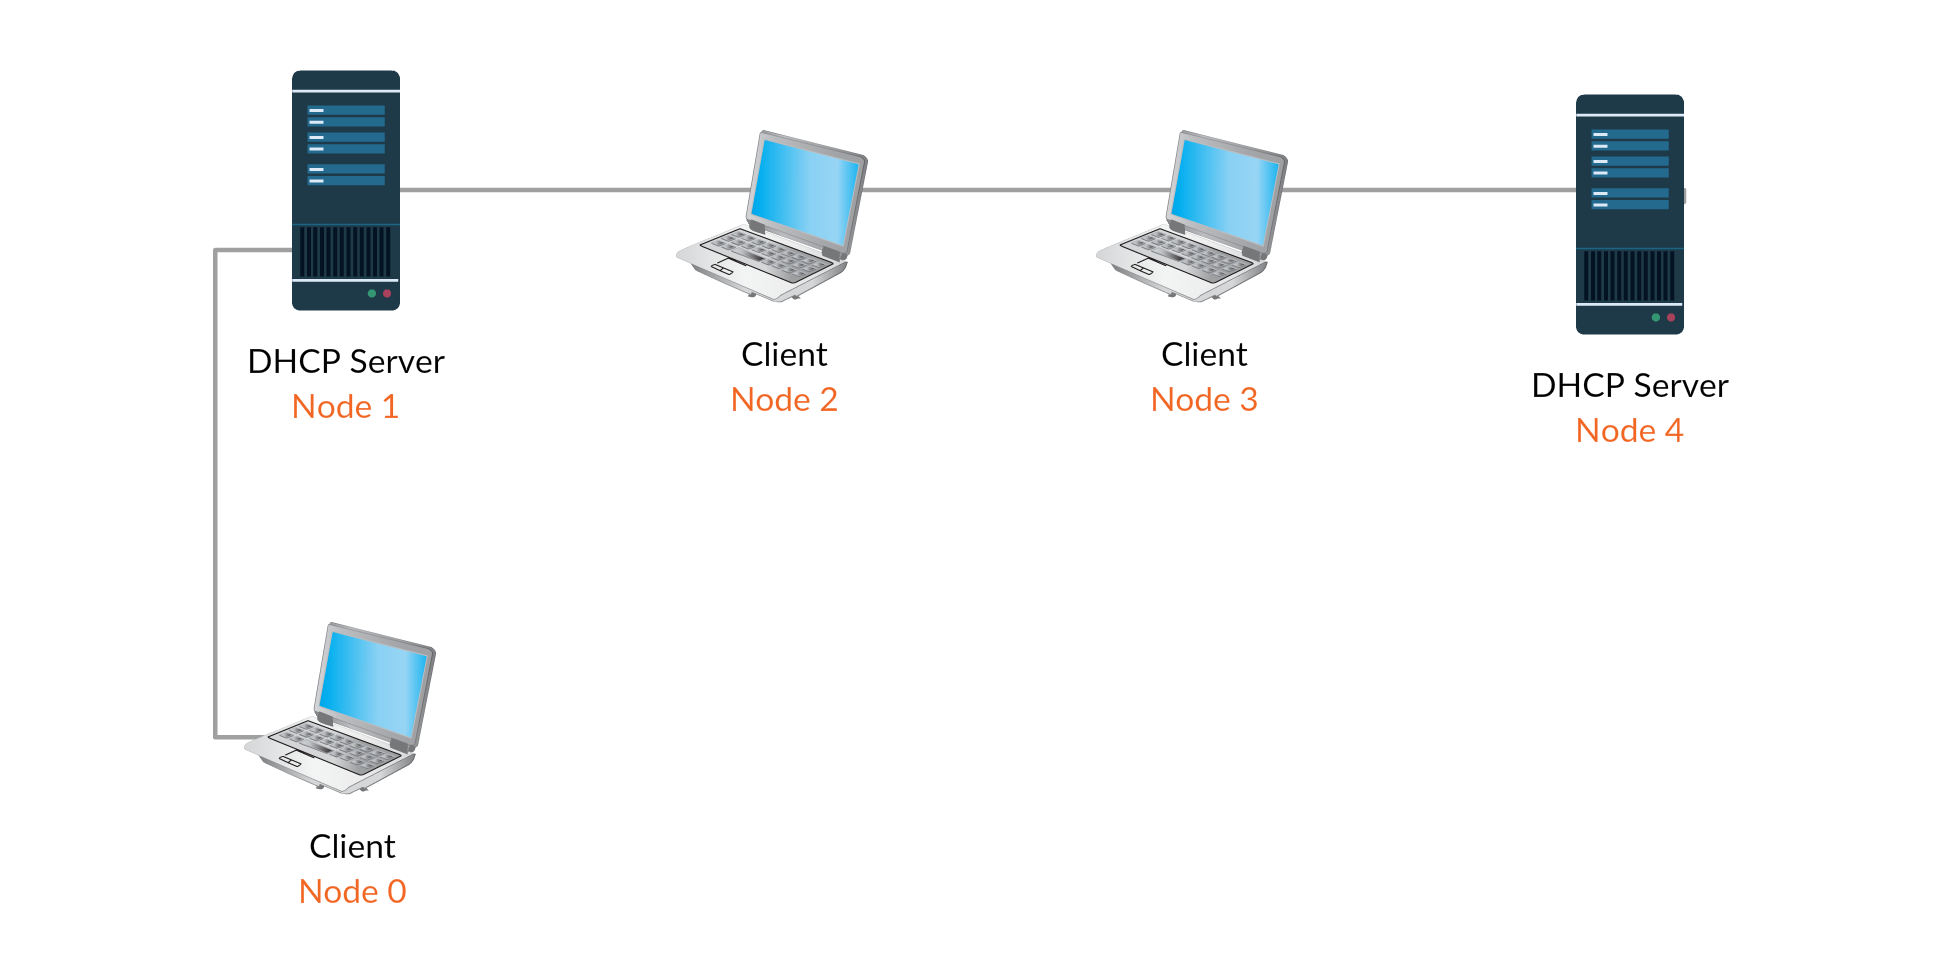
\includegraphics[scale=.4]{DHCP_Simple.png}
	\end{center}
\end{figure}

% \clearpage
{\LARGE  \textbf{نکات ضروری}}
\begin{itemize}
\item
به علت اینکه نمره‌ی تمرین به صورت خودکار داده می‌شود، ساختار پیام‌های
مطرح‌ شده باید دقیقاً به صورتی باشد که در مستند توضیح داده شده است. 
\item
نقشه‌ای که برای ارزیابی استفاده می‌شود با نقشه تست که در اختیار شما قرار گرفته متفاوت خواهد بود. 
\item
داوری خودکار به صورت کامل در اختیار شما قرار داده می‌شود و می‌توانید نمره خود را ببینید. اما ملاک ارزیابی نمره‌ای است که کد ارسالی شما روی کارگزار  خواهد گرفت. اگر موارد گفته شده را رعایت کرده باشید، نمره شما نباید تغییری داشته باشد.
\item
به دلیل مشکلات اینترنتی بهتر است داوری را هنگامی که به شبکه‌ی دانشگاه متصل هستید انجام دهید.
\item
در صورتی‌که هر مشکل یا پرسشی داشتید که فکر می‌کنید پاسخ آن برای همه مفید خواهد بود،
	آن را به گروه اینترنتی درس ارسال کنید.
\item
از فرستادن جواب تمرین به گروه اینترنتی درس خودداری کنید.
\item
 تمام برنامه‌ی شما باید توسط خود شما نوشته شده باشد. فرستادن کل یا قسمتی
	از برنامه‌تان برای افراد دیگر، یا استفاده از کل یا قسمتی از برنامه‌ی فرد دیگری، حتی با
	ذکر منبع، تقلب محسوب می‌شود.
\item
 پس از اتمام کارتان لازم است با اجرای دستور
\code{make archive}
فایل زیپی شامل تمام فایل‌هایی که برای اجرا شدن کد شما نیاز است بسازید.(این دستور فایل info.sh شما را درون زیپ قرار نمی‌دهد زیرا نیازی به این فایل نیست!) در صورتی که از کلاس‌ها و فایل‌های اضافه شده خودتان استفاده می‌کنید، سعی کنید در پوشه گفته شده باشد. در هر صورت فایل آرشیو شما باید قابلیت کامپایل/اجرا شدن را به روش سیستمی داشته باشد، در غیر اینصورت نمره شما صفر خواهد شد.
\item
نسخه نهایی تمرین خود را به
\href{http://quera.ir/}{
وب‌سایت کوئرا
}
ارسال نمایید.
\end{itemize}

\end{document}
